\chapter{Die Benutzeroberfl\"ache}
Dieses Kapitel soll die Konzeption der Oberfl�che begr�nden und deren Nutzung erl�utern.\\

\section{Anforderungen}
Die Benutzeroberfl�che muss die folgenden, aus der Problemstellung resultierenden Funktionalit�ten erf�llen:
\begin{enumerate}
	\item W�hlen, Festlegen und �ndern des Suchverzeichnisses
	\item Ausw�hlen der Keywords
	\item Ausw�hlen der Freitextsuche
	\item Eingabe des Suchtextes
	\item Logische Operatoren zur externen Verkn�pfung zur Verf�gung stellen
	\item Logische Operatoren  zur internen Verkn�pfung zur Verf�gung stellen
	\item Anzeigen der Anfrage
	\item Starten der Suche
	\item Zur�cksetzen der Anfrage
	\item Anzeige der Resultate 

	
\end{enumerate}

Neben den oben genannten inhaltlichen Anforderungen sind noch weitere Punkte bez�glich Anwenderfreundlichkeit zu ber�cksichtigen: \\
\begin{enumerate}
\item �bersichtlichkeit
\item Intuitive Bedienbarkeit, d.h. der Nutzer soll m�glichst wenig nachdenken m�ssen
\end{enumerate}

Die Realisierung  der soeben beschriebenen Anforderungen wird in den folgenden Abschnitten erl�utert.

\section{Grundaufbau der Oberfl�che}
Die Oberfl�che wurde, um dem Nutzer eine gewisse �bersichtlichkeit zu bieten, in drei Bereiche gegliedert, die in Abbildung \ref{overview} gezeigt sind. \\
Der oberste Bereich beinhaltet die Verzeichnisauswahl, da dies der erste Schritt ist, der vom Anwender ausgef�hrt werden muss.\\
In der Mitte befindet sich die Anzeige der Gesamtanfrage, weil sie sich dort sofort im Blickfeld des Nutzers befindet. \\
Die Editierung der Teilanfragen wurde im unteren Teil der Oberfl�che untergebracht, weil sich hier die meisten Bedienungselemente befinden, weshalb jede andere Position unweigerlich Einbu�en  bez�glich �bersichtlichkeit zur Folge h�tte. \\
Funktional zusammengeh�rige Elemente wurden hierbei stets nah beieinander angeordnet, was dem Gesetz der N�he entspricht. \\
Dieses Gesetz besagt, dass Elemente, die nah zusammen liegen, vom Anwender als zusammengeh�rig wahrgenommen werden (\cite{Hofer:17}, S.17).
\begin{figure} [http]
	\centering
	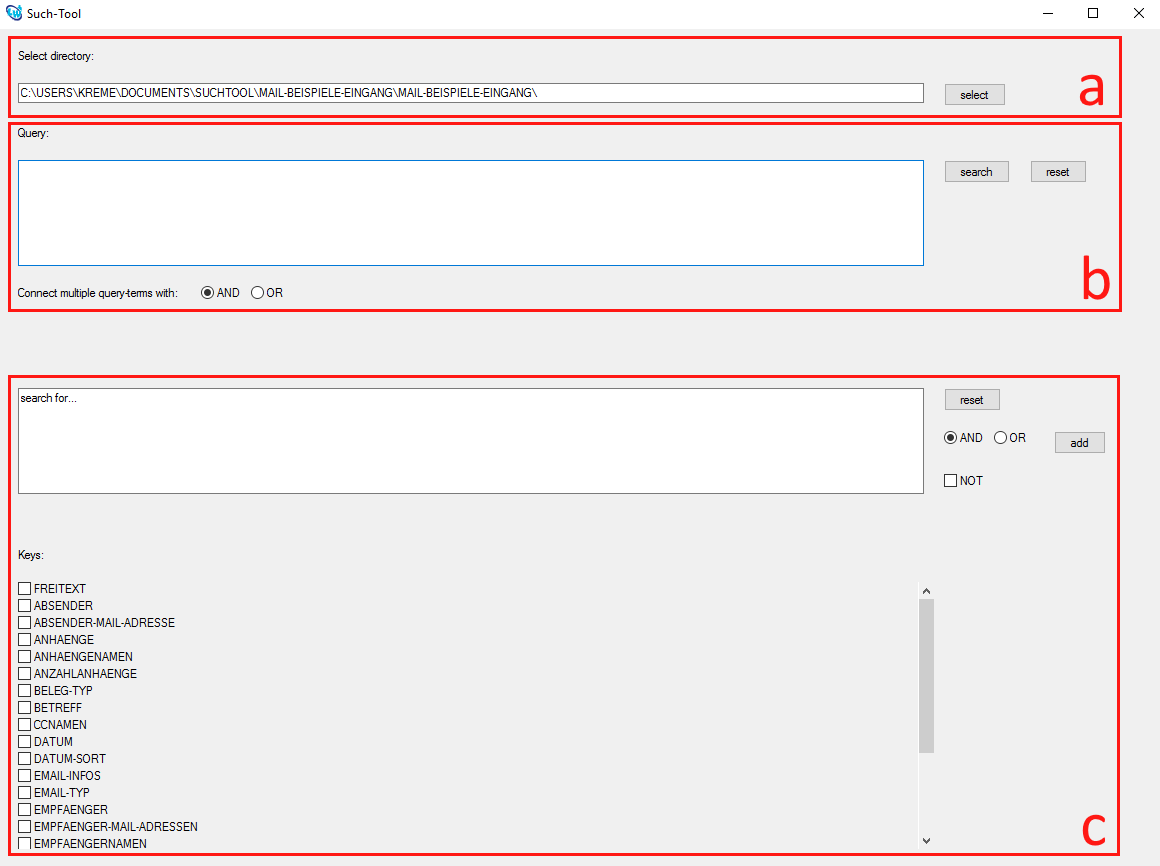
\includegraphics[width=1\textwidth]{images/overview.png}
	\caption{Gliederung der Benutzeroberfl�che. Teil \textit{a} beinhaltet die Verzeichnisauswahl, Teil \textit{b} die gesamte Suchanfrage und Teil\textit{c} die Eingabe der Teilanfrage (Eigene Abbildung).}
	\label{overview}
	
\end{figure}

\section{Verzeichnisauswahl}


\begin{figure} [http]
	
	\centering
	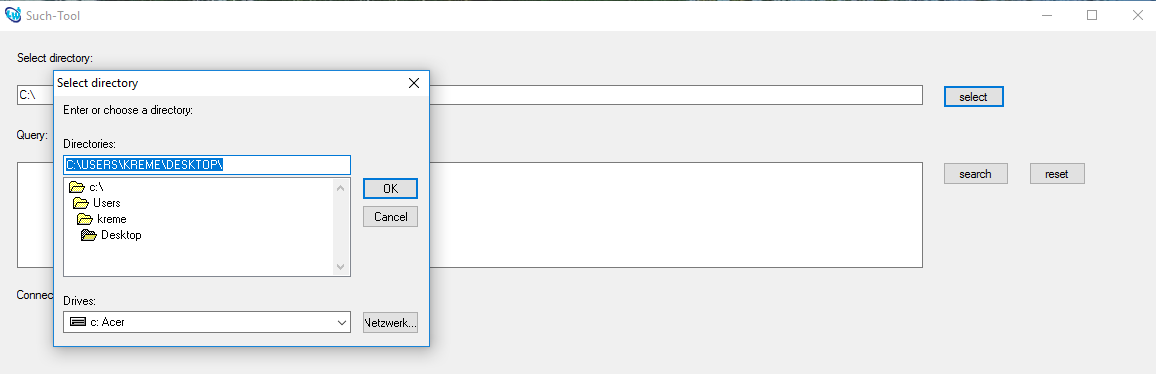
\includegraphics[width=1\textwidth]{images/Select.png}
	\caption{Verzeichnisauswahl (Eigene Abbildung)}
	\label{select}
	
\end{figure}

\section{Suchanfrage}
\begin{figure} [http]
	
	\centering
	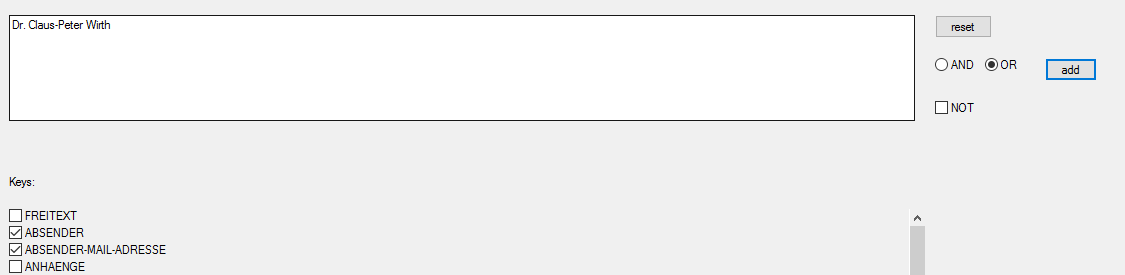
\includegraphics[width=1.1\textwidth]{images/a}
	\caption{Keywords ausw�hlen und intern verkn�pfen, hier OR (eigene Abbildung)}
	\label{a}
	
\end{figure}

\begin{figure} [http]
	
	\centering
	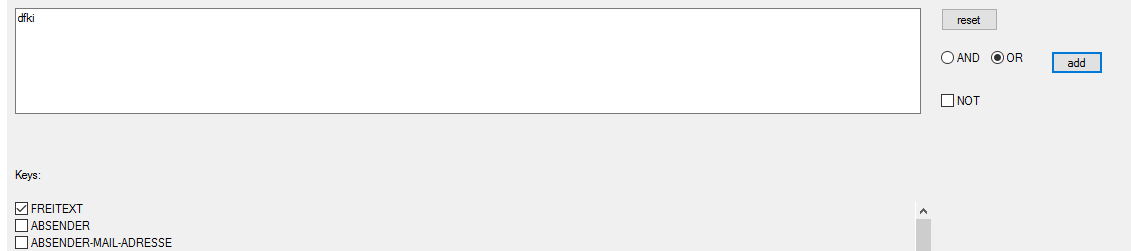
\includegraphics[width=1.1\textwidth]{images/b2}
	\caption{Keywords mit Freitext verkn�pfen (eigene Abbildung)}
	\label{b}
	
\end{figure}

\begin{figure} [http]
	
	\centering
	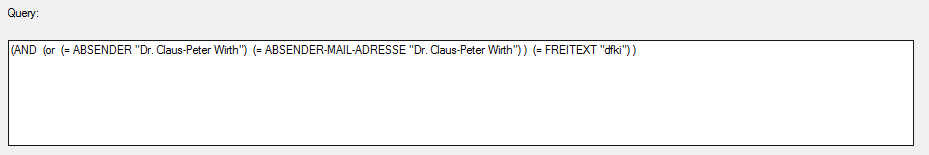
\includegraphics[width=1.1\textwidth]{images/b}
	\caption{Display (eigene Abbildung)}
	\label{c}
	
\end{figure}

\section{Ergebnis}
\begin{figure} [http]
	
	\centering
	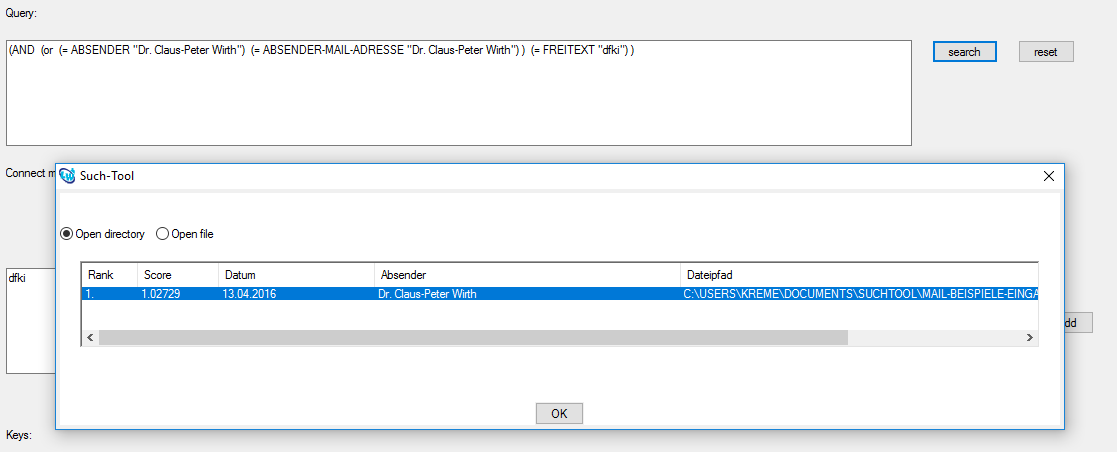
\includegraphics[width=1.1\textwidth]{images/c}
	\caption{Resultatfenster f�r obige Anfrage (eigene Abbildung)}
	\label{d}
	
\end{figure}

\begin{figure} [http]
	
	\centering
	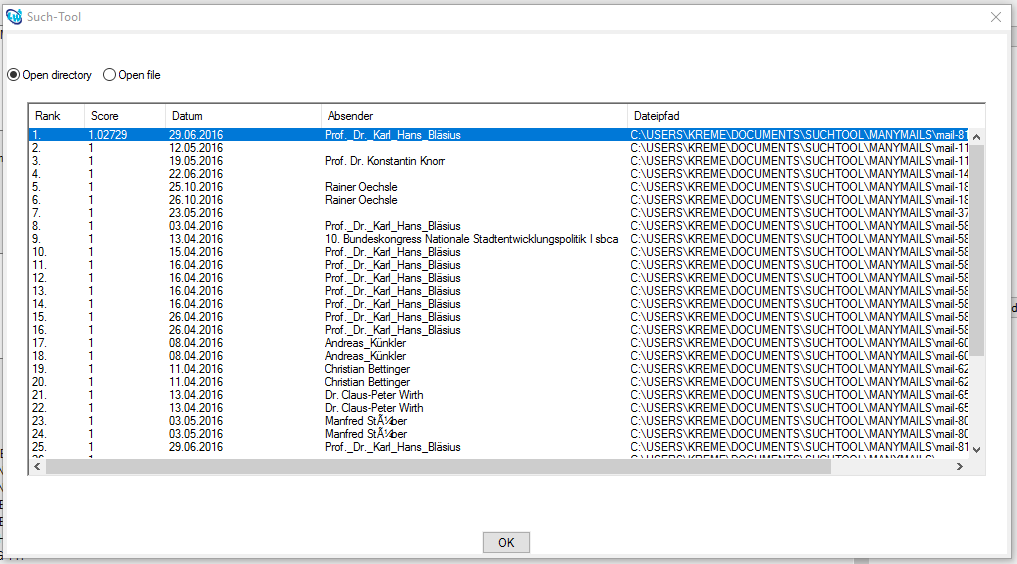
\includegraphics[width=1.1\textwidth]{images/results}
	\caption{Scrollbare Anzeige f�r viele Treffer (eigene Abbildung)}
	\label{res}
	
\end{figure}